\documentclass[a4paper,11pt]{report}

\usepackage{amsmath,amssymb,amsthm}
\usepackage{fullpage}
\usepackage{graphicx}

\usepackage{bussproofs}
\usepackage{mathpartir}
\usepackage{prooftrees}
\usepackage{color}
\usepackage{rotating}



\usepackage{tikz}
\usetikzlibrary{automata,positioning}
\usetikzlibrary{fit}

\newcommand*\circled[1]{\tikz[baseline=(char.base)]{
    \node[shape=circle,draw,inner sep=2pt] (char) {#1};}}

\makeatletter
\pgfmathdeclarefunction{alpha}{1}{%
  \pgfmathint@{#1}%
  \edef\pgfmathresult{\pgffor@alpha{\pgfmathresult}}%
}

\newcommand*{\until}{U}
\newcommand*{\disj}{\ ,\ }
\newcommand*{\A}{\square}  % Always
\newcommand*{\D}{\diamondsuit} % eventually

\newcommand*{\Pq}{(\top,\bot)}
\newcommand*{\pQ}{(\bot,\top)}
\newcommand*{\PQ}{(\top,\top)}
\newcommand*{\pq}{(\bot,\bot)}


% tikz
\usepackage{tikz}
\usetikzlibrary{snakes}


\author{Sylvain Julmy}
\date{\today}

\setlength{\parindent}{0pt}
\setlength{\parskip}{2.5pt}

\newtheorem*{thm}{Theorem}

\begin{document}

\begin{center}
  \Large{
    Automata on Infinite Structure\\
    Fall 2018
  }
  
  \noindent\makebox[\linewidth]{\rule{\linewidth}{0.4pt}}
  Exercice Sheet 10

  \vspace*{1cm}

  Author : Sylvain Julmy
  \noindent\makebox[\linewidth]{\rule{\linewidth}{0.4pt}}

  \begin{flushleft}
    Professor : Ultes-Nitsche Ulrich
    
    Assistant : Stammet Christophe
  \end{flushleft}

  \noindent\makebox[\linewidth]{\rule{\textwidth}{1pt}}
\end{center}

\section*{Exercise 1}

\begin{mathpar}
  \phi = \forall x.(x \in Q_a) \\
  x \in X_0 \implies x \in Q_a \\
  x \not\in X_0 \implies x \in Q_b \\\\
  \forall x.(x \in Q_a) \implies \forall x.(x \in X_0) \implies \\
  \forall X_1.(sing(X_1) \to X_1 \subseteq X_0) = \forall X_1.(\neg (sing(X_1)
  \vee X_1 \subseteq X_0)) =
  \\ \neg \exists \neg X_1.(\neg (sing(X_1) \vee X_1 \subseteq X_0)) =
  % \\ \neg \exists X_1 . (sing(X_1) \vee X_1 \subseteq X_0)
\end{mathpar}

\subsection*{Automata for $L_1 = X_1 \subseteq X_0$}
\begin{center}
  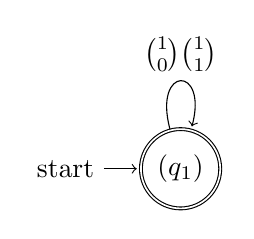
\begin{tikzpicture}[shorten >=1pt,node distance=2.5cm,on grid,auto]
    \tikzset{rounded/.style={draw,rectangle,rounded corners}}
    \node[state,initial,accepting] (q1) {$(q_1)$};
    \path[->]
    (q1)
    edge [loop above] node [above] {$\binom{1}{0}\binom{1}{1}$} ()
    ;
  \end{tikzpicture}
\end{center}

\subsection*{Automata for $L_2 = sing(X_1)$}
\begin{center}
   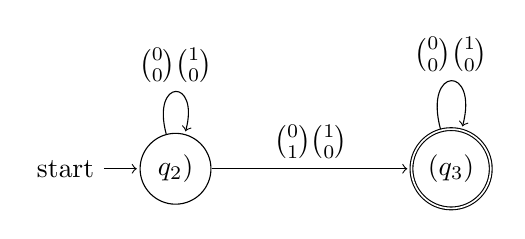
\begin{tikzpicture}[shorten >=1pt,node distance=2.5cm,on grid,auto]
    \tikzset{rounded/.style={draw,rectangle,rounded corners}}
    \node[state,initial] (q2) {$q_2)$};
    \node[state,accepting] (q3) [right = 3.5cm of q2] {$(q_3)$};
    \path[->]
    (q2)
    edge [loop above] node [] {$\binom{0}{0}\binom{1}{0}$} ()
    edge [] node [] {$\binom{0}{1}\binom{1}{0}$} (q3)
    (q3)
    edge [loop above] node [] {$\binom{0}{0}\binom{1}{0}$} ()
    ;
  \end{tikzpicture}
\end{center}

\subsection*{Automata for $L_1 \cup L_2$}

\begin{center}
  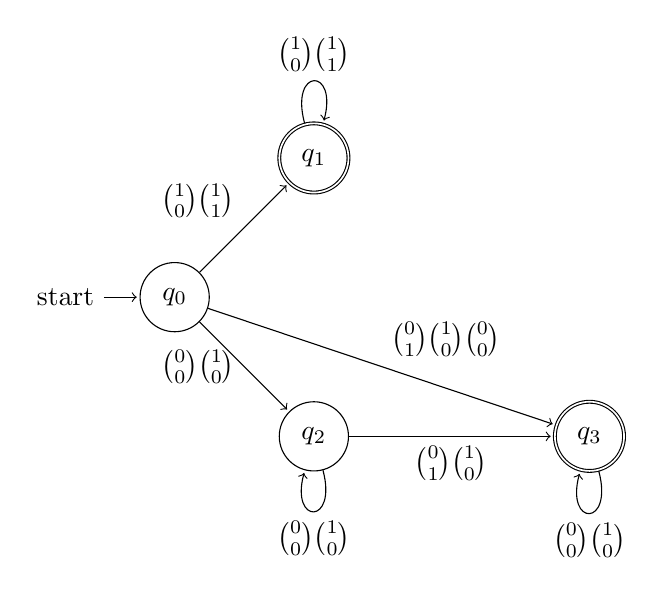
\begin{tikzpicture}[shorten >=1pt,node distance=2.5cm,on grid,auto]
    \tikzset{rounded/.style={draw,rectangle,rounded corners}}
    \node[state,initial] (q0) {$q_0$};
    \node[state,accepting] (q1) [above right = of q0] {$q_1$};
    \node[state,] (q2) [below right = of q0]{$q_2$};
    \node[state,accepting] (q3) [right = 3.5cm of q2] {$q_3$};
    \path[->]
    (q0)
    edge [] node [] {$\binom{1}{0}\binom{1}{1}$} (q1)
    edge [] node [left] {$\binom{0}{0}\binom{1}{0}$} (q2)
    edge [] node [] {$\binom{0}{1}\binom{1}{0}\binom{0}{0}$} (q3)
    (q1)
    edge [loop above] node [above] {$\binom{1}{0}\binom{1}{1}$} ()
    (q2)
    edge [loop below] node [] {$\binom{0}{0}\binom{1}{0}$} ()
    edge [] node [below] {$\binom{0}{1}\binom{1}{0}$} (q3)
    (q3)
    edge [loop below] node [] {$\binom{0}{0}\binom{1}{0}$} ()
    ;
  \end{tikzpicture}
\end{center}


\subsection*{Automata for $\overline{L_1 \cup L_2}$}

Upper part :

\begin{center}
  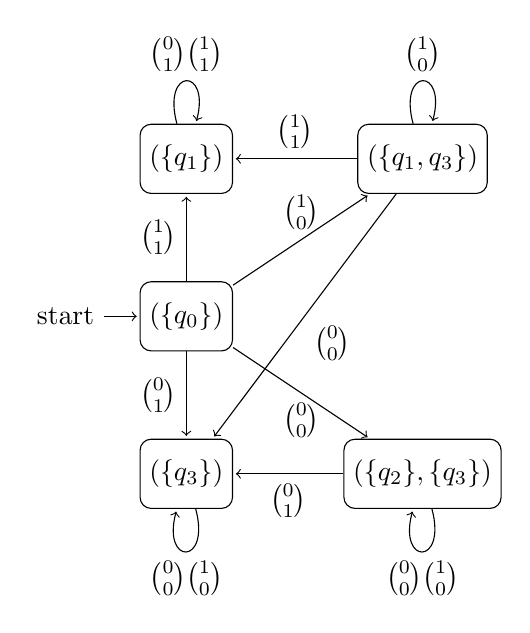
\begin{tikzpicture}[shorten >=1pt,node distance=2cm,on grid,auto]
    \tikzset{rounded/.style={draw,rectangle,rounded corners}}
    \node[state,initial,rounded] (q0) {$(\{q_0\})$};
    \node[state,rounded] (q1) [above = of q0] {$(\{q_1\})$};
    \node[state,rounded] (q3) [below = of q0] {$(\{q_3\})$};
    \node[state,rounded] (q13) [right = 3cm of q1] {$(\{q_1,q_3\})$};
    \node[state,rounded] (q23) [right = 3cm of q3] {$(\{q_2\},\{q_3\})$};
    \path[->]
    (q0)
    edge [] node [] {$\binom{1}{1}$} (q1)
    edge [] node [left] {$\binom{0}{1}$} (q3)
    edge [] node [above] {$\binom{1}{0}$} (q13)
    edge [] node [below] {$\binom{0}{0}$} (q23)
    (q1)
    edge [loop above] node [] {$\binom{0}{1}\binom{1}{1}$} ()
    (q3)
    edge [loop below] node [] {$\binom{0}{0}\binom{1}{0}$} ()
    (q13)
    edge [loop above] node [] {$\binom{1}{0}$} ()
    edge [] node [above] {$\binom{1}{1}$} (q1)
    edge [] node [] {$\binom{0}{0}$} (q3)
    (q23)
    edge [loop below] node [] {$\binom{0}{0}\binom{1}{0}$} ()
    edge [] node [] {$\binom{0}{1}$} (q3)
    ;
  \end{tikzpicture}
\end{center}

Full automata :

\begin{center}
  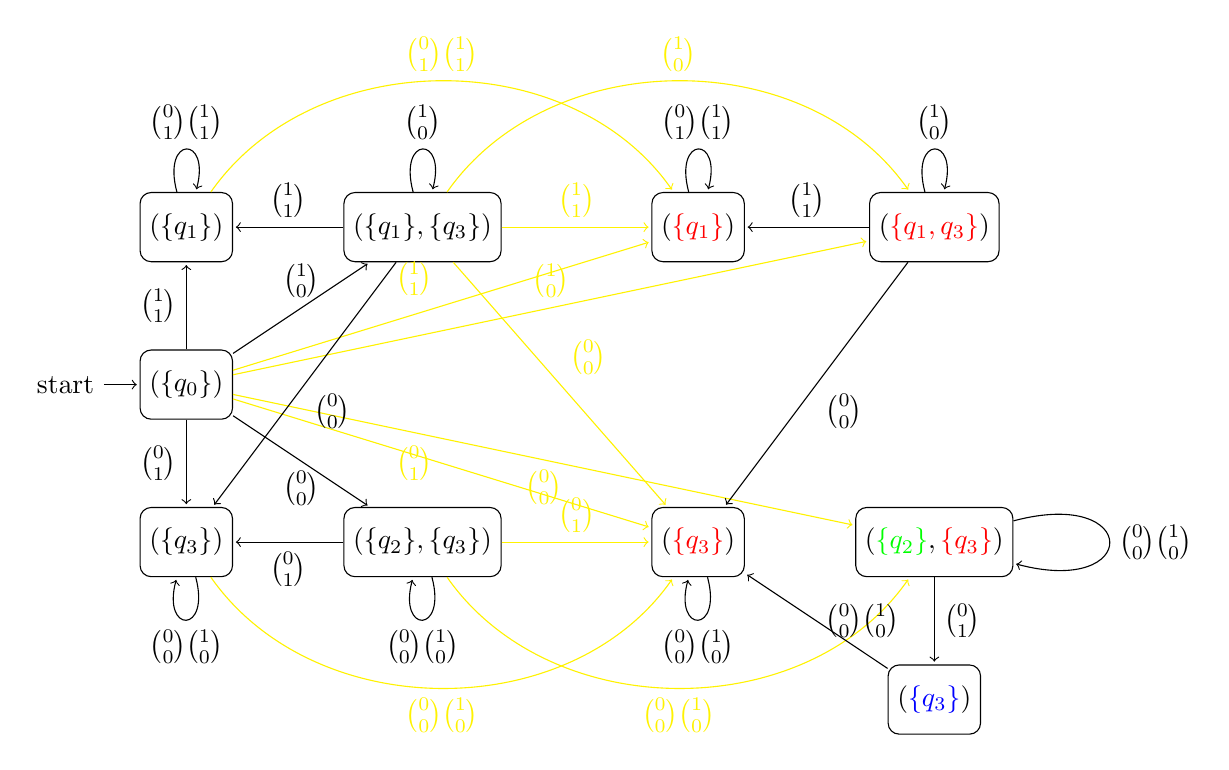
\begin{tikzpicture}[shorten >=1pt,node distance=2cm,on grid,auto]
    \tikzset{rounded/.style={draw,rectangle,rounded corners}}
    \node[state,initial,rounded] (q0) {$(\{q_0\})$};
    \node[state,rounded] (q1) [above = of q0] {$(\{q_1\})$};
    \node[state,rounded] (q3) [below = of q0] {$(\{q_3\})$};
    \node[state,rounded] (q13) [right = 3cm of q1] {$(\{q_1\},\{q_3\})$};
    \node[state,rounded] (q23) [right = 3cm of q3] {$(\{q_2\},\{q_3\})$};
    
    \node[state,rounded] (q1b) [right = 3.5cm of q13] {$(\textcolor{red}{\{q_1\}})$};
    \node[state,rounded] (q3b) [right = 3.5cm of q23] {$(\textcolor{red}{\{q_3\}})$};
    \node[state,rounded] (q13b) [right = 3cm of q1b] {$(\textcolor{red}{\{q_1,q_3\}})$};
    \node[state,rounded] (q23b) [right = 3cm of q3b] {$(\textcolor{green}{\{q_2\}},\textcolor{red}{\{q_3\}})$};

    \node[state,rounded] (q3c) [below = of q23b] {$(\textcolor{blue}{\{q_3\}})$};
    
    \path[->]
    (q0)
    edge [] node [] {$\binom{1}{1}$} (q1)
    edge [] node [left] {$\binom{0}{1}$} (q3)
    edge [] node [above] {$\binom{1}{0}$} (q13)
    edge [] node [below] {$\binom{0}{0}$} (q23)
    
    edge [yellow] node [] {$\binom{1}{1}$} (q1b)
    edge [yellow] node [left] {$\binom{0}{1}$} (q3b)
    edge [yellow] node [above] {$\binom{1}{0}$} (q13b)
    edge [yellow] node [below] {$\binom{0}{0}$} (q23b)
    (q1)
    edge [loop above] node [] {$\binom{0}{1}\binom{1}{1}$} ()
    
    edge [yellow, bend left = 55] node [] {$\binom{0}{1}\binom{1}{1}$} (q1b)
    (q3)
    edge [loop below] node [] {$\binom{0}{0}\binom{1}{0}$} ()
    
    edge [yellow, bend right = 55] node [below] {$\binom{0}{0}\binom{1}{0}$} (q3b)
    (q13)
    edge [loop above] node [] {$\binom{1}{0}$} ()
    edge [] node [above] {$\binom{1}{1}$} (q1)
    edge [] node [] {$\binom{0}{0}$} (q3)
    
    edge [yellow] node [above] {$\binom{1}{1}$} (q1b)
    edge [yellow, bend left = 55] node [above] {$\binom{1}{0}$} (q13b)
    edge [yellow] node [] {$\binom{0}{0}$} (q3b)
    (q23)
    edge [loop below] node [] {$\binom{0}{0}\binom{1}{0}$} ()
    edge [] node [] {$\binom{0}{1}$} (q3)
    
    edge [yellow, bend right = 55] node [below] {$\binom{0}{0}\binom{1}{0}$} (q23b)
    edge [yellow] node [] {$\binom{0}{1}$} (q3b)
    
    (q1b)
    edge [loop above] node [] {$\binom{0}{1}\binom{1}{1}$} ()
    (q3b)
    edge [loop below] node [] {$\binom{0}{0}\binom{1}{0}$} ()
    (q13b)
    edge [loop above] node [] {$\binom{1}{0}$} ()
    edge [] node [above] {$\binom{1}{1}$} (q1b)
    edge [] node [] {$\binom{0}{0}$} (q3b)
    (q23b)
    edge [loop right] node [] {$\binom{0}{0}\binom{1}{0}$} ()
    edge [] node [] {$\binom{0}{1}$} (q3c)
    (q3c)
    edge [] node [right] {$\binom{0}{0}\binom{1}{0}$} (q3b)
    ;
  \end{tikzpicture}
\end{center}

There are no accepting state...which seems weird and indicates that I have made
a mistake...

\section*{Exercise 2}

\begin{figure}[ht]
  \centering
  \includegraphics[width=0.9\textwidth]{ex2}
\end{figure}

\begin{figure}[ht]
  \centering
  \includegraphics[width=0.9\textwidth]{ex2b}
\end{figure}


\end{document}